\section{606 --- Construct String from Binary Tree}
You need to construct a string consists of parenthesis and integers from a binary tree with the preorder traversing way.

The null node needs to be represented by empty parenthesis pair \(\). And you need to omit all the empty parenthesis pairs that don't affect the one-to-one mapping relationship between the string and the original binary tree.

\paragraph{Example 1:}

\begin{flushleft}
\textbf{Input}:
\begin{figure}[H]
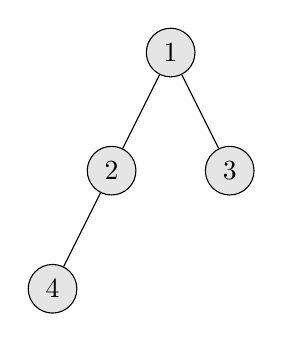
\begin{tikzpicture}
[every node/.style={draw, circle, fill=gray!20!, minimum size=5mm}]
\node{1}
child{node{2} child{node{4}} child[missing]}
child{node{3}};
\end{tikzpicture}
\end{figure}

\textbf{Output}: $ 1(2(4))(3) $

\textbf{Explanation}: 

Originally it needs to be $ 1(2(4)())(3()()) $, 

but you need to omit all the unnecessary empty parenthesis pairs. 

And it will be $ 1(2(4))(3) $.
\end{flushleft}

\paragraph{Example 2:}
\begin{flushleft}

\textbf{Input}:
\begin{figure}[H]
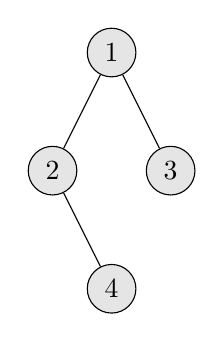
\begin{tikzpicture}
[every node/.style={draw, circle, fill=gray!20!, minimum size=5mm}]
\node{1}
child{node{2} child[missing] child{node{4}}}
child{node{3}};
\end{tikzpicture}
\end{figure}

\textbf{Output}: $ 1(2()(4))(3) $

\textbf{Explanation}: 

Almost the same as the first example, 

except we can't omit the first parenthesis pair to break the one-to-one mapping relationship between the input and the output.
\end{flushleft}